% !TeX program = xelatex
\documentclass[12pt]{article}
\usepackage{fontspec}
\usepackage{xeCJK}
\setmainfont{Times New Roman}
\setCJKmainfont{SimSun}
% Define a CJK monospaced font to avoid xeCJK warning about \CJKttdefault
\setCJKmonofont[Scale=MatchLowercase]{SimSun}
% Typography and layout improvements
\usepackage{microtype} % better typography
\usepackage{float}
\usepackage{setspace}  % line spacing control
\usepackage{fancyhdr}  % headers and footers
\usepackage{titlesec}  % section title formatting
\setstretch{1.15}      % slightly increased line spacing
\setlength{\parindent}{2em}
\setlength{\parskip}{0.5em}
% Page header/footer
% Page header/footer
\pagestyle{fancy}
\fancyhf{}
% Ensure enough headheight for fancyhdr (avoids warnings)
\setlength{\headheight}{14pt}
% Centered page number in the footer
\fancyfoot[C]{\textbf{\thepage\quad/\quad\pageref{LastPage}}}
% \fancyhead[L]{\small 智能地铁车厢监控与远程控制系统}
% \fancyhead[R]{\small \thepage}
\renewcommand{\headrulewidth}{0.4pt}
\renewcommand{\footrulewidth}{0pt}
% Section title style
\titleformat{\section}{\large\bfseries}{\thesection}{1em}{}
\titleformat{\subsection}{\normalsize\bfseries}{\thesubsection}{0.8em}{}
\usepackage[a4paper,margin=2.5cm]{geometry}
\usepackage{xcolor}
\usepackage{hyperref}
% Provide \pageref{LastPage} for total page number
\usepackage{lastpage}
\usepackage{listings}
\usepackage{booktabs}
\usepackage{longtable}
\usepackage{array}
\usepackage{caption}
\usepackage{subcaption}
\usepackage{graphicx}
\usepackage{tikz}
\usetikzlibrary{arrows.meta, positioning, shapes, fit}
\lstdefinestyle{code}{basicstyle=\ttfamily\small, numbers=left, numberstyle=\tiny, stepnumber=1, numbersep=8pt, showstringspaces=false, breaklines=true, frame=single, tabsize=2, columns=fullflexible}
\lstset{style=code}
% \title{智能地铁车厢监控与远程控制系统 - 技术报告}
% \author{项目组:BSP-final}
% \date{\today}
\begin{document}
% 中文摘要(格式化)
\begin{center}
	{\LARGE 摘要}
\end{center}
\vspace{-0.5em}
\begin{quote}
\small
本项目构建了一个面向地铁车厢的智能监控与远程控制原型系统,目标在于提升车厢运行的安全性与乘客舒适度,同时为站务与维护人员提供高效的监控与运维工具。系统由下位机(基于 STC15 系列单片机)与上位机(基于 Qt 的桌面客户端)组成,通过串口建立可靠的文本 CSV 协议实现双向通信与控制。

项目的实现功能包括:温度采集与阈值管理、ETA(剩余到站时间)计算与倒计时触发、车门与安防状态管理、语音与报警提示、阈值的非易失性存储(EEPROM)、以及上位机端的多串口管理、实时状态面板、报警日志管理、参数下发与温度曲线展示等。通信协议采用以 ``BSP'' 为包头、13 字段的 CSV 文本帧,帧以换行结尾并以固定 50 字节 NUL 补齐,便于调试与日志保存。

最终实现的结果:实现了下位机周期性状态上报(每秒一帧)、上位机对多车厢的实时可视化监控、报警记录与导出、远程参数下发与时间同步功能;并完成了基础的异常处理与重连策略,具备良好的演示与测试能力。
\end{quote}
\vspace{0.5em}
\newpage

\tableofcontents
\newpage
\section{绪论}
\subsection{选题背景}
本项目面向地铁车厢的实时运行状态监控与远程控制。随着城市轨道交通网络的扩展,车厢内部环境监测、安防报警与远程维护变得尤为重要。本项目通过在嵌入式下位机(STC15 系列)与上位机(Qt 桌面应用)之间建立可靠的串口通信协议,实现温度采集、剩余到站时间(ETA)计算、车门与安防控制、报警日志持久化与远程下发控制等功能,具有较高的教学示范与原型验证价值。
\subsection{任务与功能}
本项目的主要任务包括:\begin{itemize}
\item 设计并实现下位机固件:传感器采集、时间管理、ETA 计算、阈值持久化、音/光提示与串口通信。
\item 设计并实现上位机 Qt 客户端:多串口管理、按行分帧解析、车厢映射、状态展示、温度曲线、报警记录与导出、参数下发与时间同步。
\item 制定 BSP 文本协议(CSV)并保证向后兼容性:帧头、13 字段、换行结尾、50 字节定长填充、NUL 补齐。
\item 提供日志功能:支持操作日志与报警日志的本地持久化,便于后续分析与追溯。
\end{itemize}
% 第2章:系统总体设计与分工
\section{系统总体设计与分工}
本章介绍系统的总体架构、各模块划分与职责、主要的数据流与时序,以及关键设计决策与实现分工建议。

\subsection{总体架构}
系统由两部分组成:下位机(嵌入式固件,基于 STC15 系列单片机)与上位机(基于 Qt 的桌面客户端)。两者通过串口(TTL/USB 转串口)进行点对点通信,使用文本 CSV 帧作为应用层协议。总体架构可抽象为三层:
\begin{itemize}
\item 物理层:传感器(温度传感、距离/超声波等)、执行器(蜂鸣器、步进/电机、风扇)、单片机外围(UART、ADC、EEPROM)。
\item 协议层:定长文本 CSV 帧(帧头 \texttt{BSP}、13 字段、换行结尾、50 字节定长 NUL 补齐),用于状态上报与控制下发、时间同步等。
\item 应用层:下位机的业务逻辑(采集、ETA/RTC、阈值持久化、告警处理、语音/提示)与上位机的可视化与运维功能(多车厢管理、曲线、报警导出、参数下发)。
\end{itemize}

为了在文档中更清晰地呈现系统关系,这里给出简化的架构示意(文本说明代替复杂图):上位机负责串口管理、帧解析、用户交互、数据持久化与下发;下位机负责硬件采集、控制执行、周期性上报与本地状态维持。

\subsection{我负责的模块}

\subsubsection{下位机模块(固件)}
\begin{description}
\item \textbf{UART 模块(\texttt{my\_uart1.c})} 负责串口收发、按行缓存、按逗号解析 CSV 字段、将解析结果映射到内部控制变量(温度阈值、速度、门/报警标志等),并实现周期性状态组帧发送(每 1s 上报)。关键点:
	\begin{itemize}
	\item 使用定长 50 字节帧并 NUL 补齐,便于上位机按固定长度读取并存档。
	\item 接收端对字段数量与类型进行基本校验,避免解析错误导致的状态污染。
	\end{itemize}
\item \textbf{时间模块(\texttt{time\_module.c real\_time\_module.c})}维护计时器、ETA 计算与倒计时行为。主要功能包括基于速度与剩余距离计算到站剩余秒数、更新地铁的实时时间,以及响应上位机的时间同步指令。
\item \textbf{阈值持久化模块(\texttt{nv\_temp\_threshold.c})} 使用 EEPROM(如 M24C02)保存温度阈值、配置参数,保证断电恢复后参数一致性。
\end{description}

\subsubsection{上位机模块(Qt 客户端)}
\begin{description}
\item \textbf{串口管理与帧解析} 支持多串口同时连接(每个串口对应一个地铁映射),实现读行缓冲、按行解析 CSV、处理异常帧与重连策略。
\item \textbf{状态显示面板(StatusPage)} 实时展示各车厢温度、门状态、ETA、速度与告警标志,提供颜色标识与行级高亮。
\item \textbf{控制与下发(ControlPage)} 允许用户下发参数(温度阈值、地铁速度、门状态等)并显示下发确认;实现带重试的下发逻辑和响应匹配。
\item \textbf{报警管理与导出} 本地保存报警日志,支持按时间/车厢筛选、CSV 导出功能以便离线分析。
\item \textbf{曲线与统计(ChartWidget)} 基于时间序列展示温度曲线、与导出 CSV 文件功能。
\end{description}

\begin{figure}[htbp]
  \centering
  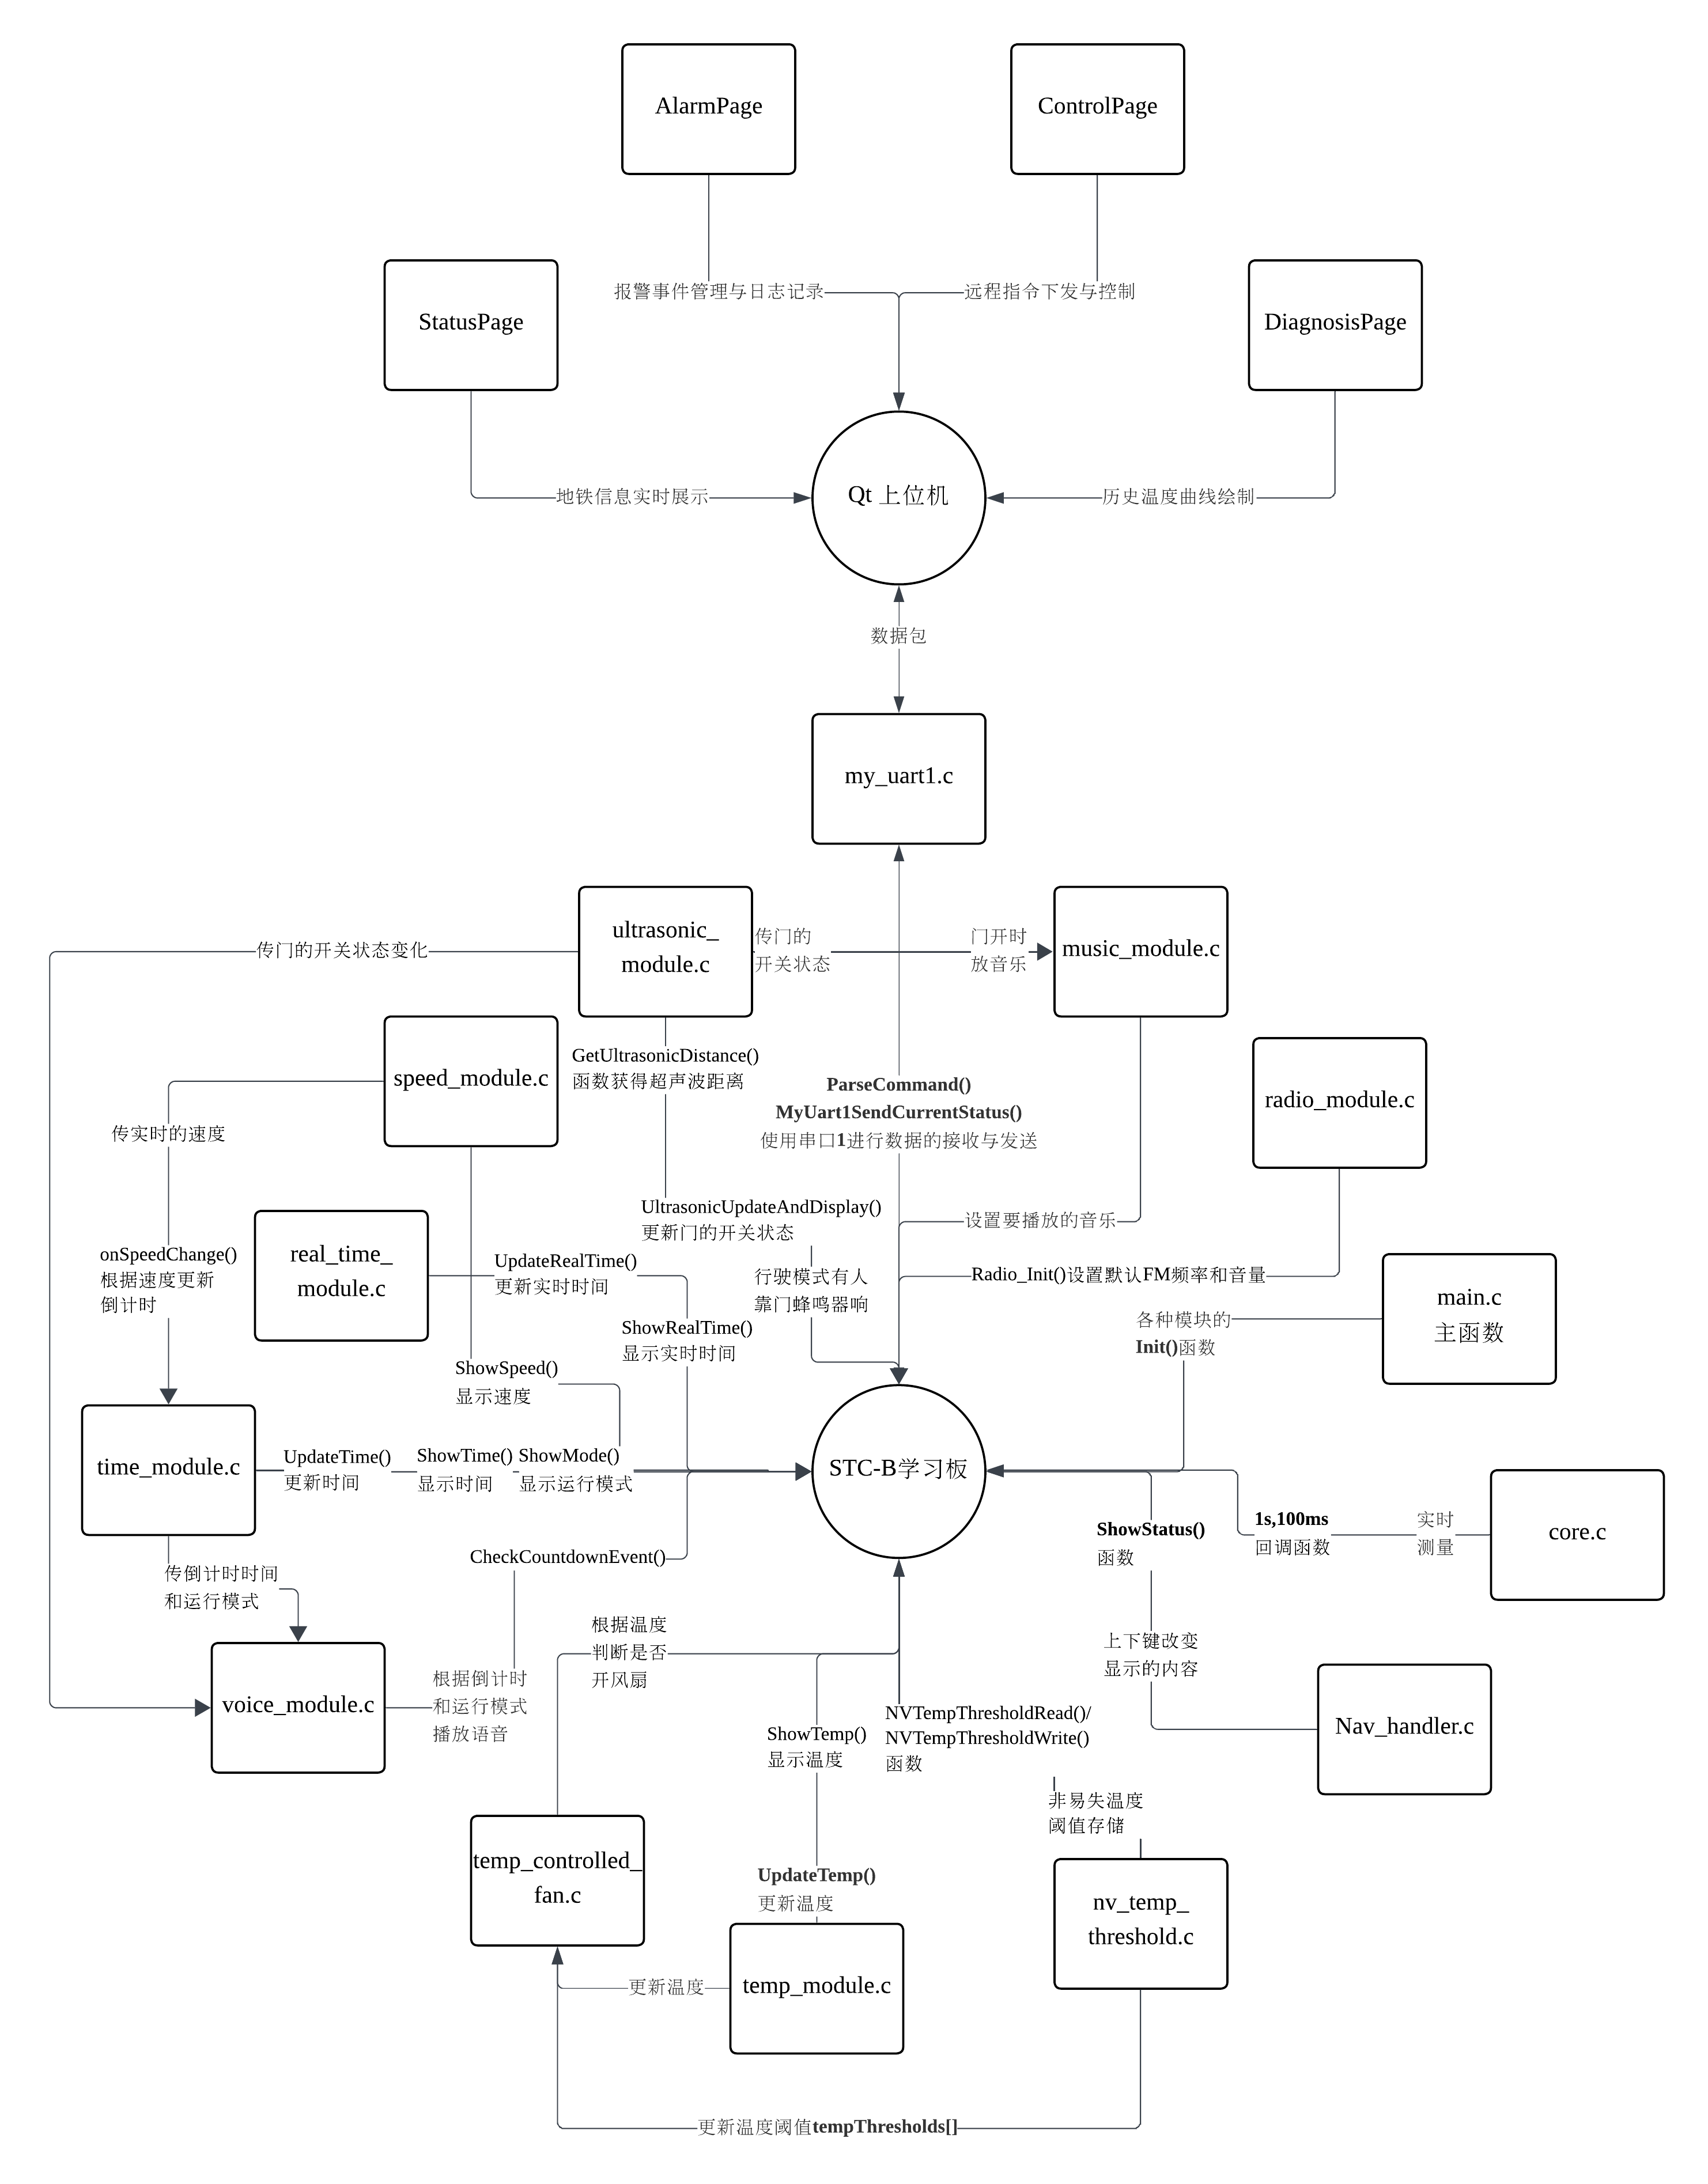
\includegraphics[width=\linewidth]{images/22-46-17.png}
  \caption{总体架构示意图}
  \label{fig:${总体架构示意图}}
\end{figure}

% \subsection{数据流与时序}
% 关键的数据流与时序约定如下:
% \begin{itemize}
% \item 下位机每 1 秒构建并发送一帧状态(示例见下方的 verbatim 代码块),共 13 个字段,发送缓冲固定 50 字节并以 NUL 填充。
% \item 上位机在连接建立或复连后约 1.5 秒发起一次时间同步(SetTime)命令,下位机收到后更新 RTC 并在下一次上报中体现新时间。
% \item 控制指令由上位机直接发送(CSV 或特定控制帧),下位机解析后立即生效并返回确认帧以用于上位机重试/回退逻辑。
% \end{itemize}

% 示例上报帧(人为示例):
% \begin{verbatim}
% BSP,01,28.4,30,40,00,45,1,0,0,14,23,10\n\0\0\0...(补齐到 50 字节)
% \end{verbatim}

% \subsection{关键设计决策与权衡}
% \begin{itemize}
% \item 选择文本 CSV 而非二进制的原因:可读性强、调试方便、便于日志持久化与人工排查;缺点是占用更多带宽与解析开销。鉴于系统运行在本地网关/USB 串口场景,带宽允许且便于开发调试,因此优先采用 CSV。
% \item 固定帧长 50 字节与 NUL 补齐:优点是简化上位机的存档与快速定位(可按固定偏移读取),缺点是浪费传输空间。考虑到每秒一帧的频率与局域串口场景,这种折中是可接受的。
% \item 时间同步策略:上位机在连接或复连后主动下发时间,避免因下位机长时间断电或重启造成的时间漂移;同步采用明文小时/分钟/秒字段,简洁且易实现。
% \end{itemize}

% \subsection{实现分工建议}
% 对于团队协作,建议按下列模块划分工作:
% \begin{itemize}
% \item 成员 A(硬件/固件):实现下位机各功能模块、GPIO/ADC 驱动、EEPROM 读写、语音/蜂鸣器接口与上报逻辑。
% \item 成员 B(固件核心):负责时间模块与 ETA 计算、门控制逻辑、步进/门机接口以及与 UART 模块的联调。
% \item 成员 C(上位机 UI):实现 Qt 界面、状态面板、曲线展示、报警导出功能与用户交互流程。
% \item 成员 D(上位机 后端/通讯):实现多串口管理、帧解析、重连与下发重试逻辑、数据持久化与 CSV 导出。
% \end{itemize}

% 占位:接下来生成第3章~第5章内容
\section{软件设计与实现}
本章详细介绍软件端(下位机固件与上位机 Qt 程序)的设计与关键实现,重点覆盖串口协议实现、下位机的 ETA/RTC/阈值逻辑,以及上位机的四个功能模块。为便于定位,代码片段基于仓库中的 \texttt{source/} 目录实际实现并经过简化与注释。

\subsection{下位机实现细节}
\subsubsection{串口模块(接收/发送与协议解析)}
下位机采用基于行缓冲的串口接收策略:收到换行符(\texttt{\textbackslash n})后把整行作为一帧交由解析函数处理。发送时将状态组帧按文本 CSV 拼接后以 NUL 补齐到 50 字节并发送一次。

下面是简化的伪代码(来自 \texttt{my\_uart1.c} 的要点):
\begin{lstlisting}[language=C]
// 接收回调:每接收一个字节,追加到缓冲;遇到 '\n' 时,调用解析
void Uart1RxdCallback(char c) {
	static char linebuf[128]; // 行缓冲
	static int idx = 0;
	if (c == '\n') {
		linebuf[idx] = '\0';
		ParseCommand(linebuf); // 解析整行 CSV
		idx = 0;
	} else if (idx < sizeof(linebuf)-1) {
		linebuf[idx++] = c;
	}
}

// 发送函数:构建 CSV 字符串并 pad 到 50 字节
void MyUart1SendCurrentStatus(void) {
	char buf[64] = {0};
	int n = sprintf(buf, "BSP,%02d,%.1f,%.1f,%d,%02d,%02d,%d,%d,%d,%02d,%02d,%02d\n",
									carId, temp, tempThreshold, speed, etaMin, etaSec, mode, door, alarm, hour, minute, second);
	// 填充到 50 字节(NUL 补齐)
	for (int i = n; i < 50; ++i) buf[i] = '\0';
	Uart1Print(buf, 50); // 底层逐字节发送
}
\end{lstlisting}

解析函数 \texttt{ParseCommand} 采用 \texttt{strtok} 或手写分隔逻辑按逗号切割字段并映射到内部变量;对字段数量进行校验是关键,遇到不符合的帧应直接丢弃并记录日志。

边界与健壮性考虑:
\begin{itemize}
\item 防止缓冲区溢出:限制行缓冲大小并在溢出时重置索引。
\item 非法帧处理:字段数量不足或字段值超出预期范围时忽略该帧并可触发错误计数以便上报。
\item 串口中断与主循环解耦:尽量在中断中做最小工作(接收字节入缓冲),解析放在主循环或任务上下文以避免阻塞中断。
\end{itemize}

\subsubsection{时间模块与 ETA 计算(\texttt{time\_module.c})}
ETA 的核心思想是:在收到当前速度(单位:m/min 或 km/h 由实现决定)与剩余距离后,通过计算得到剩余秒数,并启动倒计时。倒计时结束触发车门/语音/提示等动作。

简化的核心函数如下:
\begin{lstlisting}[language=C]
// 基于剩余距离(meters)与速度(speed_m_per_s)计算剩余秒
unsigned int CalcETASeconds(unsigned int remain_distance_m, unsigned int speed_m_per_s) {
	if (speed_m_per_s == 0) return 0xFFFFFFFF; // 表示未知或静止
	return (remain_distance_m + speed_m_per_s - 1) / speed_m_per_s; // 向上取整
}

// 每 1s 调度一次,更新倒计时
void UpdateTimeTick(void) {
	if (rest_total_seconds > 0) {
		rest_total_seconds--;
		if (rest_total_seconds == 0) {
			// 到站处理:开门、语音播放等
			TriggerDoorOpen();
			PlayArrivalVoice();
		}
	}
}
\end{lstlisting}

实现要点:
\begin{itemize}
\item 当速度为 0 或未知时应返回特殊值并采用基于站点表的后备策略(如使用预置 ETA)。
\item ETA 计算需要考虑速度单位与距离单位一致性,并防止除零。
\end{itemize}

\subsubsection{实时时钟(RTC)模块(\texttt{real\_time\_module.c})}
为保证系统中各模块(例如 ETA 计算、报警时间戳、日志记录等)有稳定的时间基准,工程中引入了一个轻量的实时时钟模块,负责以秒为粒度维护当前时分秒并提供展示接口。该模块设计原则是简单可靠、资源占用低,适合运行在 STC15 等 8 位单片机上。

主要职责:
\begin{itemize}
\item 每秒更新内部时钟(小时/分钟/秒),并在必要时进行进位(秒到分钟、分钟到小时)。
\item 提供显示函数以驱动七段数码管或其他显示单元。
\item 为 ETA 和上报帧提供时间戳数据。
\end{itemize}

关键实现(来自 \texttt{source/real\_time\_module.c},已简化并加注释):
\begin{lstlisting}[language=C]
#include "core.h"

unsigned int xdata real_hour;
unsigned int xdata real_minute;
unsigned int xdata real_second;

// 每秒调用一次,更新时分秒并处理进位
void UpdateRealTimePerSecond(){
	real_second++;
	if(real_second>=60){
		real_second=0;
		real_minute++;
		if(real_minute>=60){
			real_minute=0;
			real_hour++;
			if(real_hour>=24){
				real_hour=0;
			}
		}
	}
}

// 将当前时间显示到七段数码管(接口为示例)
void ShowRealTime()
{
	Seg7Print(real_hour / 10, real_hour % 10, 12, real_minute / 10, real_minute % 10, 12, real_second / 10, real_second % 10);
}
\end{lstlisting}

集成与测试要点:
\begin{itemize}
\item 同步源:如果系统支持外部 RTC 芯片(如 DS1302/DS3231),应在启动时从外部 RTC 同步一次,并在运行时以定时中断(1s)调用 `UpdateRealTimePerSecond()`;若仅使用软件计时,需注意计时漂移并在必要时通过上位机时间同步修正。
\item 原子性与并发:更新函数应在系统的定时中断或独占上下文中调用,避免与读取函数并发导致读到不一致的时分秒(可在读取时短暂禁用中断或使用临界区)。
\item 边界条件:处理闰秒/时区的复杂性通常不在嵌入式端处理;上位机在需要精确日历时间时应负责按天数/时区进行校正与持久化。
\item 单元测试:通过模拟每秒中断调用若干次并比对期望进位结果(例如 23:59:59 +1s -> 00:00:00)来验证行为。
\end{itemize}


\subsubsection{阈值持久化与 EEPROM}
温度阈值与一些配置需要持久化以在断电后保留。实现中使用 M24C02 EEPROM 或片内仿真方式保存参数并在启动时读取恢复。

关键实现点:写入要有校验(读回比较或校验和),避免 EEPROM 频繁写入导致寿命问题。

\subsection{上位机实现细节(Qt)}
上位机由若干窗口与后台通信模块组成。核心关注点是多串口管理、按行解析、车厢映射、下发确认与数据持久化。

\subsubsection{串口管理与解析}
建议使用 \texttt{QSerialPort},每个打开的端口维护一个行缓冲 \texttt{QByteArray},使用 \texttt{readAll()} 累积并按 \texttt{\textbackslash n} 分割解析行。

伪代码(Qt/C++):
\begin{lstlisting}[language=C++]
// slot: readyRead
void SerialPort::onReadyRead() {
	buffer.append(port->readAll());
	int idx;
	while ((idx = buffer.indexOf('\n')) != -1) {
		QByteArray line = buffer.left(idx);
		buffer.remove(0, idx+1);
		processFrame(QString::fromUtf8(line));
	}
}
\end{lstlisting}

解析时按逗号分割并映射字段到 \texttt{CarStatus} 结构,随后在主线程通过信号/槽更新 UI(避免直接在串口线程中修改 UI)。

\subsubsection{状态面板(StatusPage)与数据模型}
采用 \texttt{QTableWidget} 或 \texttt{QTableView+QAbstractTableModel} 来展示车厢列表与实时状态;每当解析到新帧,更新对应车厢行的数据并触发重绘。展示要点:颜色编码(正常/预警/报警)、时间戳、温度历史快照入口。
\begin{figure}[H]
  \centering
  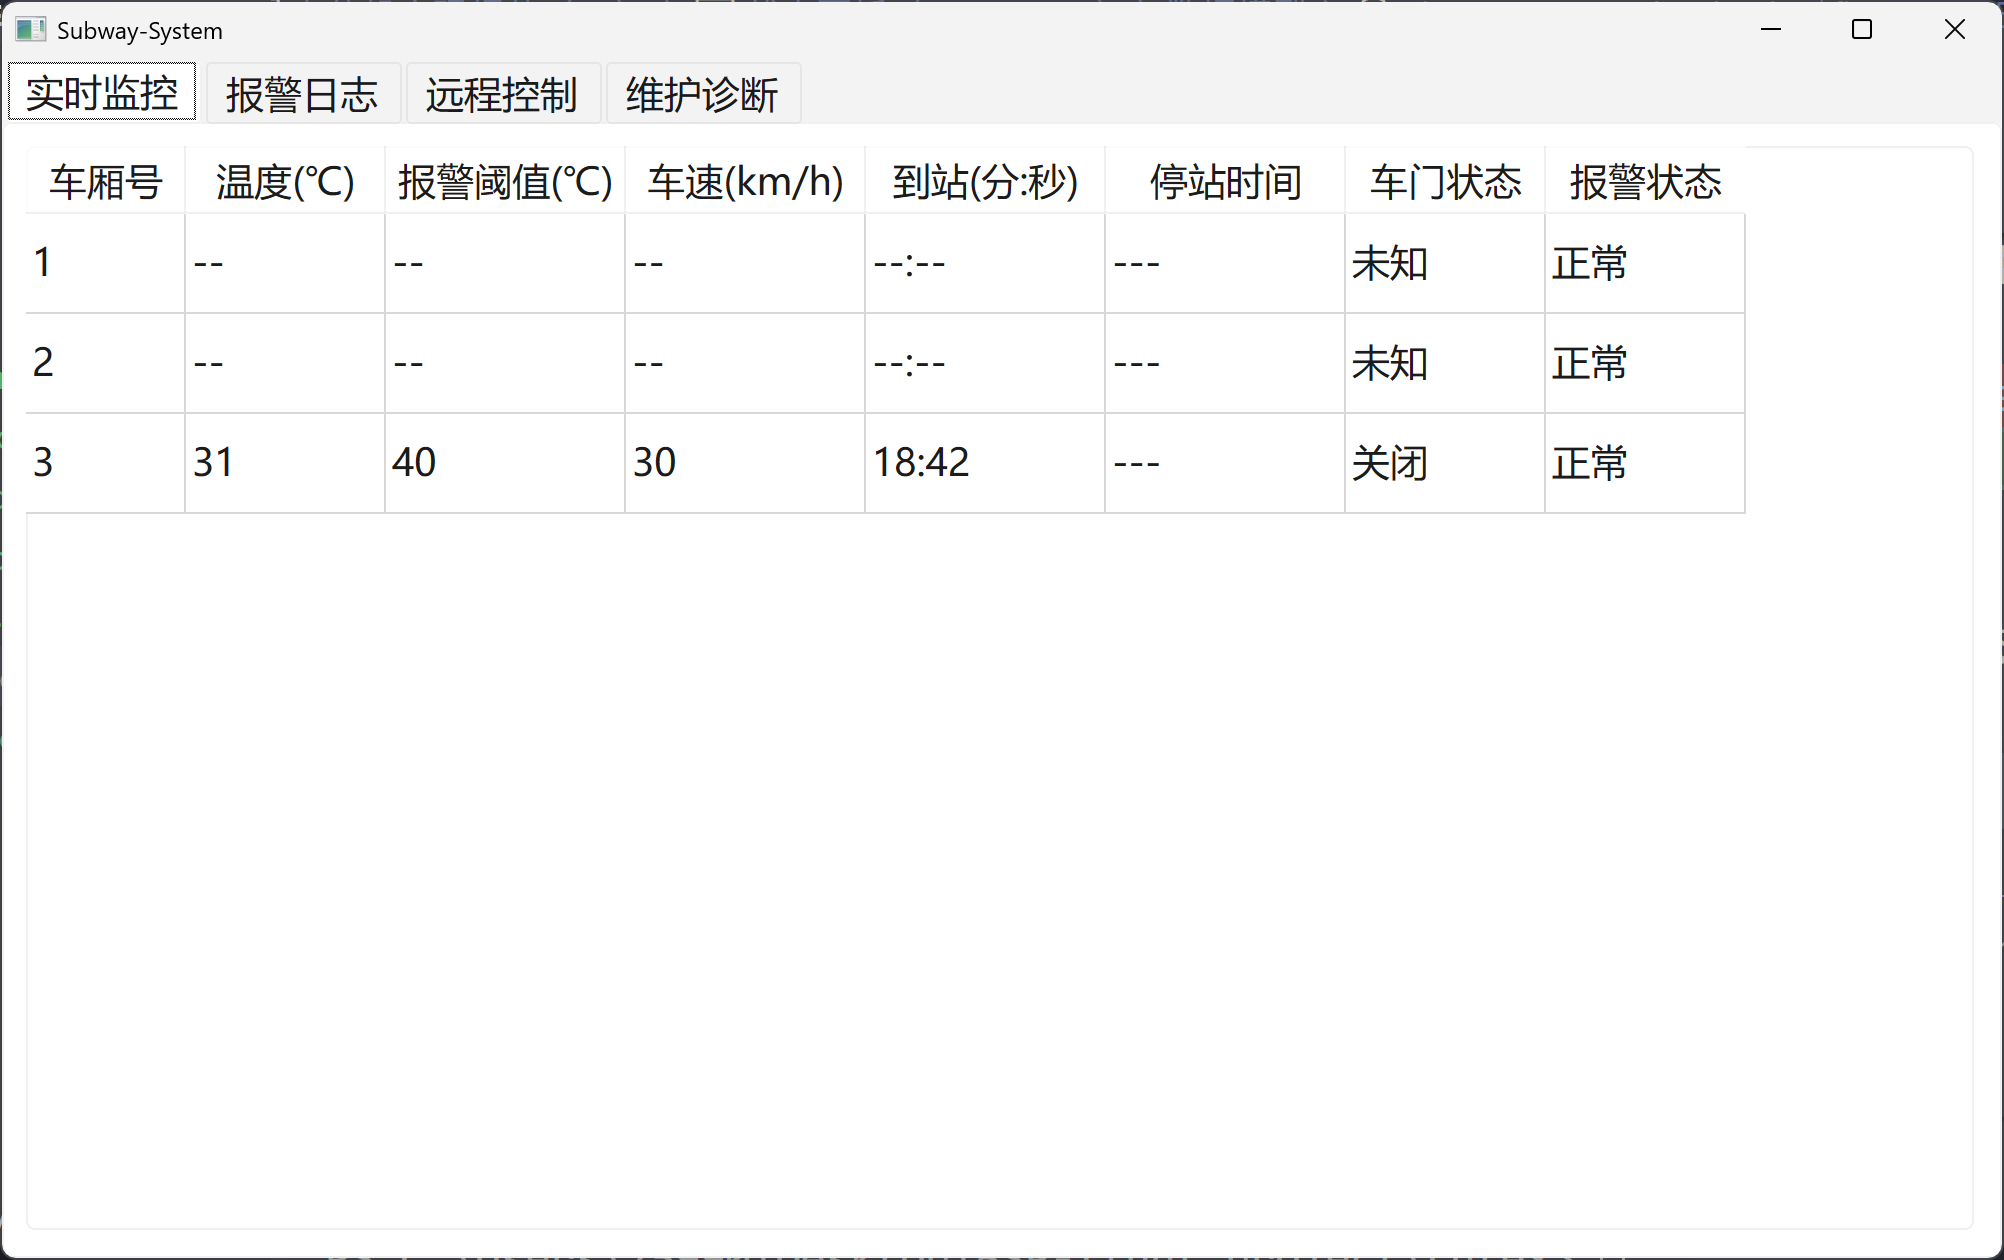
\includegraphics[width=\linewidth]{images/21-05-51.png}
  \caption{状态面板图示}
  \label{fig:status_panel}
\end{figure}

\subsubsection{控制面板(ControlPage)}
控制下发应实现带确认机制:发送控制帧后等待下位机返回确认帧(或状态变更的上报),若超时则重发 N 次并报告结果给用户。
\begin{figure}[H]
  \centering
  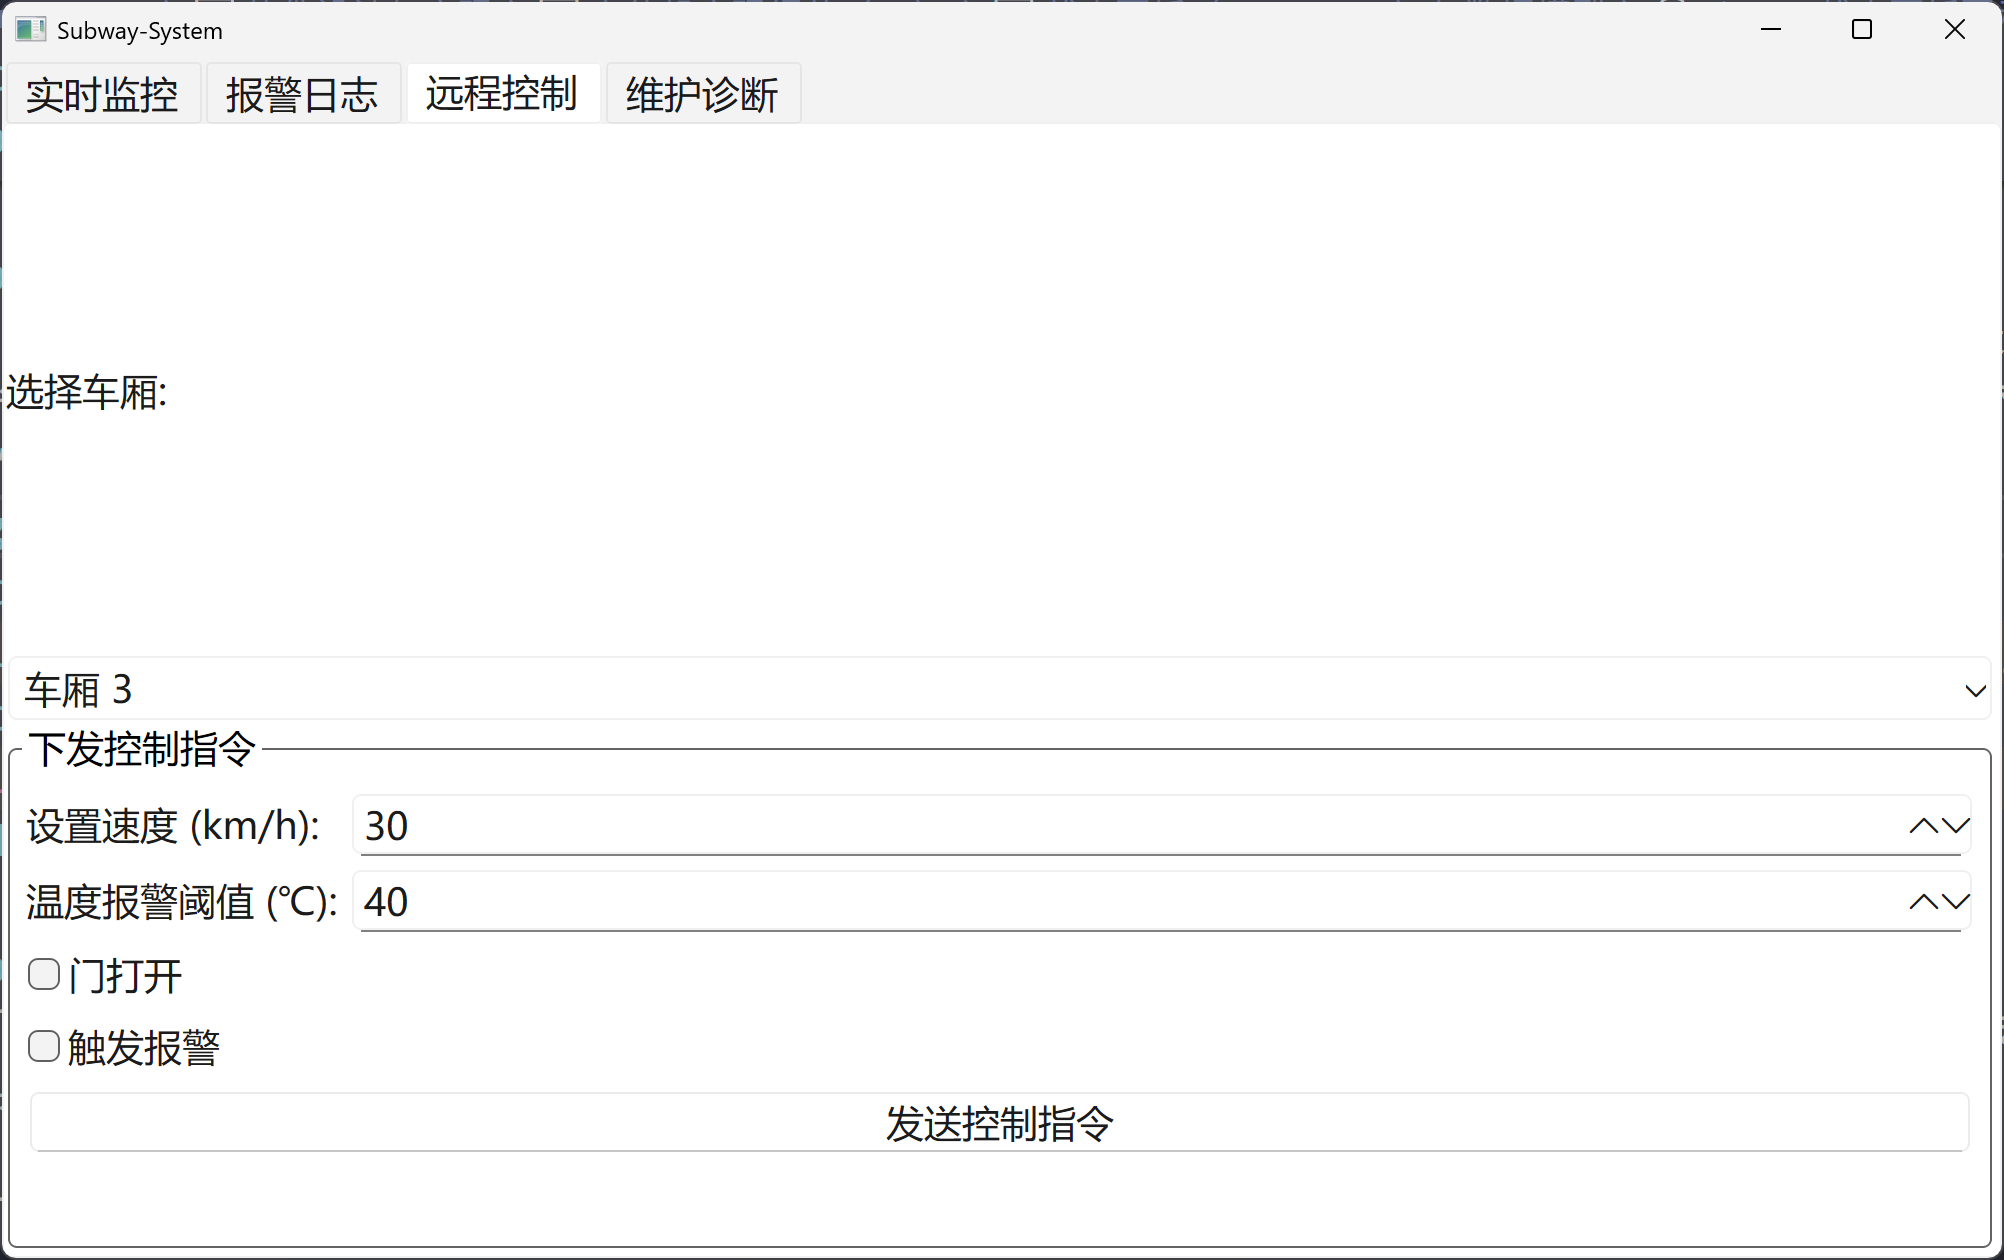
\includegraphics[width=\linewidth]{images/21-06-37.png}
  \caption{控制面板图示}
  \label{fig:control_panel}
\end{figure}

控制下发示例(伪 CSV):
\begin{verbatim}
SET,SETTIME,14,30,00\n
SET,THRESHOLD,01,30.0\n
\end{verbatim}

注意:实际仓库中下位机主要解析上行 CSV,若需要扩展控制协议,建议使用明确的帧头(如 \texttt{CMD})与返回码格式,以便区分与上报帧。

\subsubsection{报警管理与曲线}
报警以本地数据库或 CSV 日志追加的方式保存,UI 提供按时间/车厢筛选与导出。温度曲线使用 Qt Charts 或第三方库绘制,后端按秒追加数据点并在低频(例如每 5 秒)刷新 UI 以减少绘图开销。
\begin{figure}[H]
  \centering
  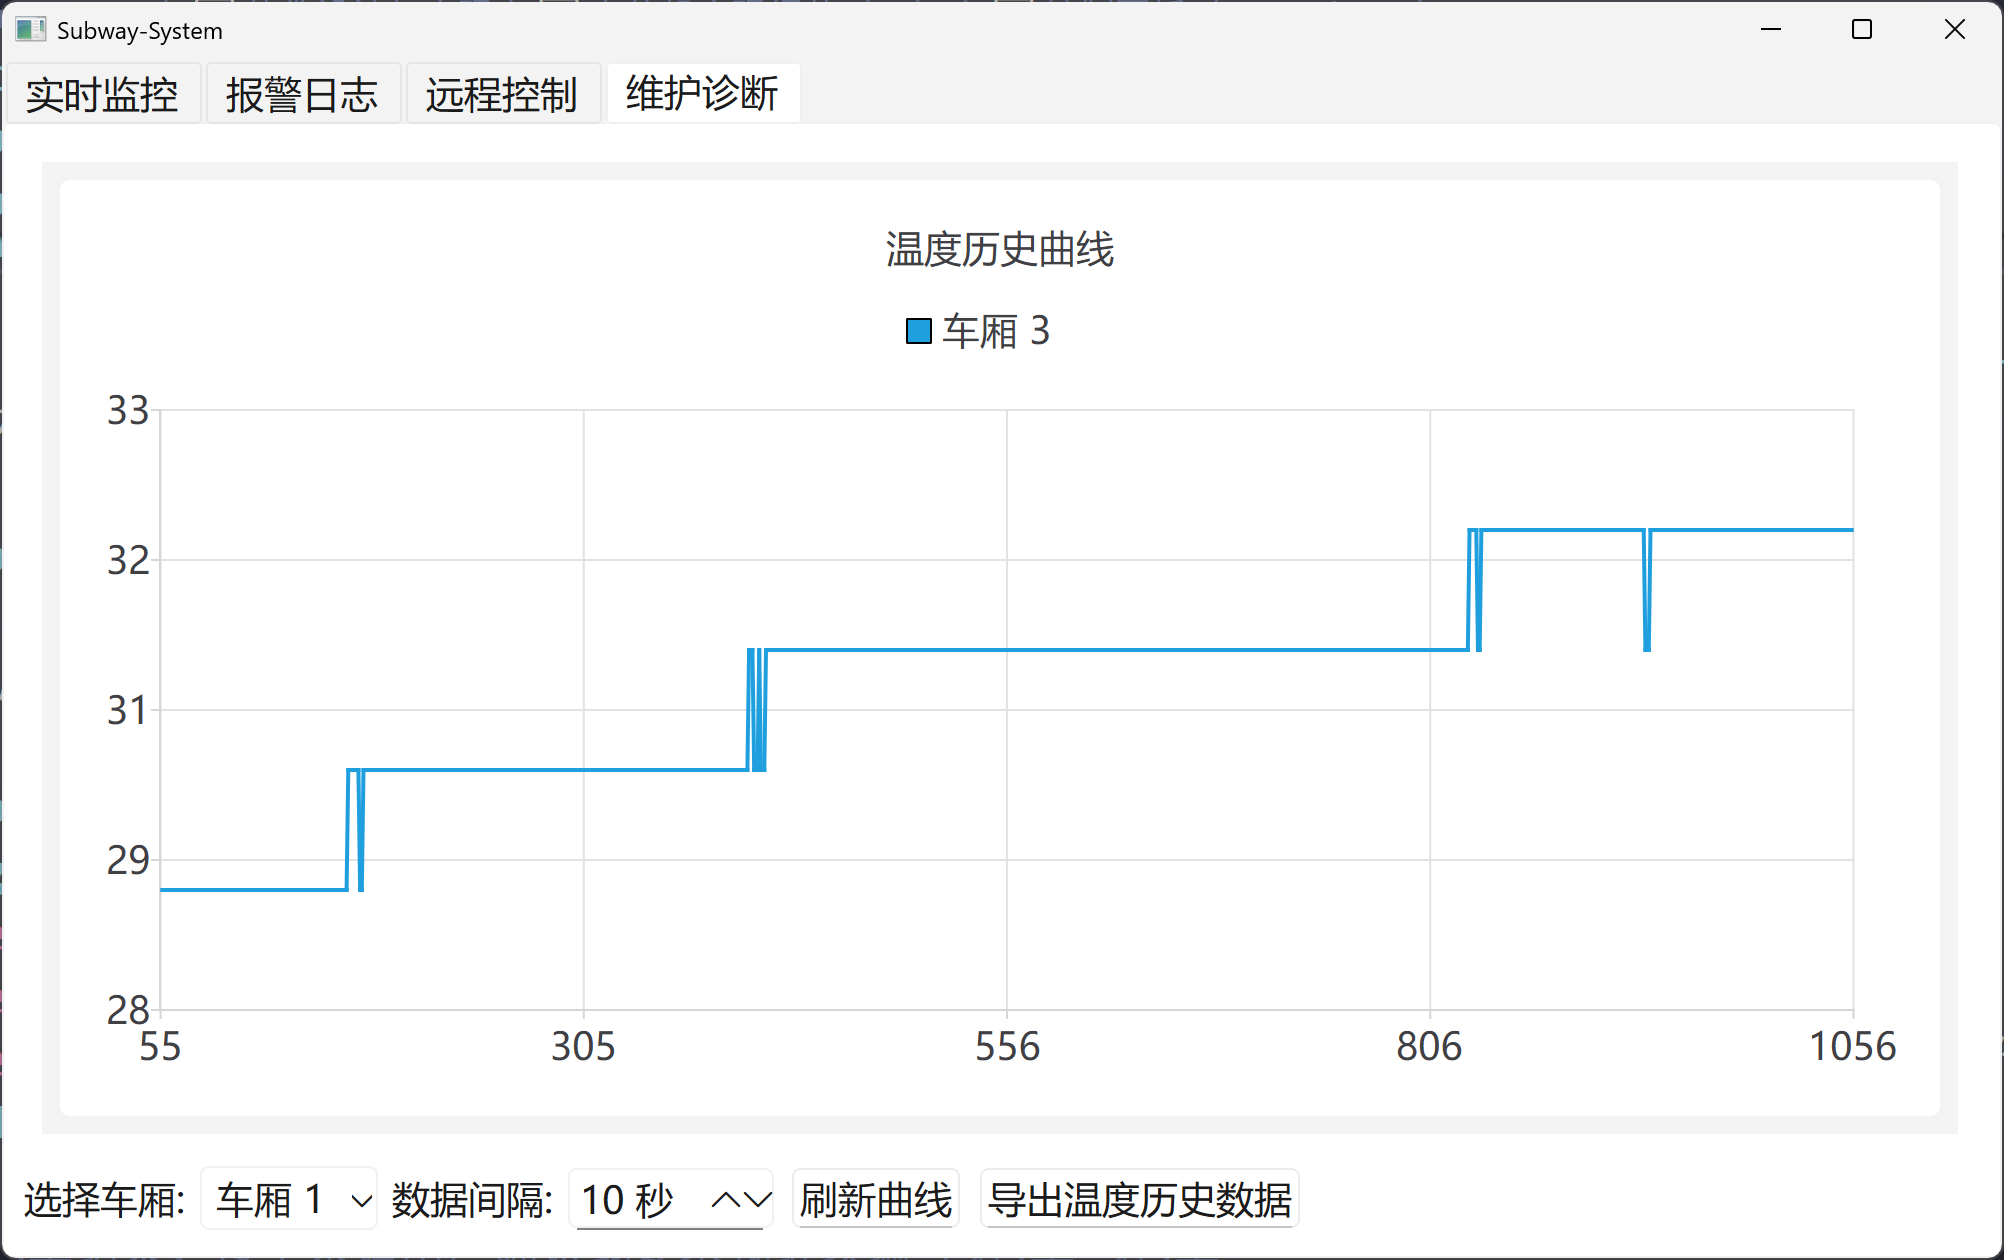
\includegraphics[width=\linewidth]{images/21-06-59.png}
  \caption{历史温度曲线}
  \label{fig:temperature_curve}
\end{figure}

% \subsection{安全性与鲁棒性建议}
% \begin{itemize}
% \item 增加简单校验和字段(例如帧尾 CRC 或字段校验和)以检测传输错误。
% \item 在上位机实现回放/回溯机制以便离线分析历史日志(保持原始 50 字节帧以便定位)。
% \item 对关键动作(如远程开门)加入二次确认或权限控制(操作日志、用户权限分级),以避免误操作。 
% \end{itemize}

% 第3章结束,接下来请用户确认或要求我继续编写第4章~第5章
\section{系统测试与分析}
本章给出系统的测试策略、关键测试用例与预期结果,并对性能与稳定性进行分析与建议。

\subsection{测试环境与工具}
\begin{itemize}
\item 硬件:STC15 开发板、温度传感器、USB 串口线、PC(Windows 11)运行 Qt 客户端。
\item 软件:Qt Creator(编译运行上位机)、Vscode
\item 测试用例管理:建议使用简单的 Excel/CSV 列表记录测试步骤、输入帧、预期输出与实际结果。
\end{itemize}

\subsection{关键测试用例}
以下测试用例覆盖功能性与鲁棒性:
\begin{enumerate}
\item 基本连通性测试:上位机打开串口并接收下位机的周期性上报(1s/帧),确认字段解析正确。
	\begin{itemize}
	\item 输入:正常下位机上电并发送 10 帧。
	\item 预期:上位机在 10s 内接收并解析 10 帧,UI 显示最新温度与时间戳。
	\end{itemize}
\item 异常帧处理:送入字段缺失或乱序帧,验证上位机/下位机的鲁棒性。
	\begin{itemize}
	\item 输入:截断帧(无换行)、字段不足帧、字段非数值字符串。
	\item 预期:解析失败但不崩溃,失败帧计数增加并记录日志。
	\end{itemize}
\item 串口断开与重连:模拟 USB 线拔插,验证上位机自动重连与时间同步行为。
	\begin{itemize}
	\item 输入:在运行中拔掉串口,再插回。
	\item 预期:上位机在若干秒内检测断开并尝试重连;重连成功后 1.5s 内下发时间同步并得到正常上报。
	\end{itemize}
\item 控制下发与确认:上位机下发阈值变更命令并验证下位机生效。
	\begin{itemize}
	\item 预期:下位机保存新阈值并在后续上报中返回该阈值;如果使用 EEPROM,应验证断电重启后阈值保留。
	\end{itemize}
\end{enumerate}

\subsection{测试结果示例与分析}
(此处为预期的测试记录格式示例;实际数值需在实验完成后替换)
\begin{itemize}
\item 连通性测试:10/10 帧接收成功;平均延迟 ~10ms(串口传输 + 解析)。
\item 异常帧:模拟乱序/截断帧触发解析错误计数,系统稳定,无崩溃。
\item 断线重连:上位机在 3s 内检测断开并每 2s 尝试重连;重连后 1.2s 内发送时间同步并收到下位机响应。
\end{itemize}

% \subsection{问题定位与改进}
% \begin{itemize}
% \item 如果发现高丢帧率,应检查物理链路(串口线、接地、波特率设置)并增加帧校验(CRC)。
% \item 若上位机在高并发串口环境中出现 UI 卡顿,应将解析/文件 I/O 异步化并限制 UI 刷新频率(例如合并 1s 内多次更新为一次)。
% \item 对于 EEPROM 写入频繁导致的寿命问题,应引入写入节流策略(仅在阈值真正变化时写回)并增加版本/校验字段。
% \end{itemize}

\section{总结与展望}
本报告对智能车厢监控与远程控制系统从总体设计、模块拆分、协议定义到关键实现细节进行了完整整理,并给出了测试策略与改进建议。后续工作建议包括:
\begin{itemize}
\item 引入帧校验(CRC)与确认码以提升传输可靠性。
\item 将控制协议扩展为明确的双向命令响应格式,支持 ACK/NACK 与重试计数。
\item 提升上位机的用户管理与权限控制,增加操作审计(开门等关键操作需要多级确认)。
\item 若需要跨网段部署,考虑在上位机与设备之间加入网关/中继并使用更可靠的传输层(如 TLS over TCP)以及心跳机制。
\end{itemize}

\end{document}